\chapter{Output}\label{output}

EnergyPlus produces several output files as shown in the section on ``Running EnergyPlus''.~~ This section will discuss the data contained in the ``standard'' output file (\textbf{eplusout.eso}).~ It, too, has a data dictionary but unlike the input files, the output data dictionary is contained within the output file.~ Thus, the basic structure of the standard output file is:

\begin{lstlisting}
Data Dictionary Information
End of Data Dictionary
Data
...
Data
End of Data
\end{lstlisting}

As with the IDF structure, there are rules associated with the interpretation of the standard output data dictionary.~ These rules are summarized as follows:

\begin{itemize}
\item
  The first item on each line is an integer which represents the ``report code''.~ This ``report code'' will be listed in the data section where it will also be the first item on each line, identifying the data.~ Only 2 lines in the output file will not have an integer as the first item (``End of Data Dictionary'' and ``End of Data'' lines).
\item
  The second item on each line is also an integer.~ This integer corresponds to the number of items left on the dictionary line.~ Each string consists of a variable name and units in square brackets.~ Square brackets are required for all strings.~ If there are no units associated with a particular variable, then there are no characters between the brackets.
\end{itemize}

Six standard items appear at the start of every EnergyPlus Standard Output File Data Dictionary:

\begin{lstlisting}
Program Version,EnergyPlus, 1.0, Beta 2, Build 017
1,5,Environment Title[],Latitude[degrees],Longitude[degrees],Time Zone[],Elevation[m]
2,6,Day of Simulation[],Month[],Day of Month[],DST Indicator[1 = yes 0 = no], Hour[], StartMinute[], EndMinute[], DayType
3,3,Cumulative Day of Simulation[],Month[],Day of Month[],DST Indicator[1 = yes 0 = no],DayType
4,2,Cumulative Days of Simulation[],Month[]
5,1,Cumulative Days of Simulation[]
\end{lstlisting}

\begin{itemize}
\item
  Item 0 is the program version statement.
\item
  Item 1 is produced at the beginning of each new ``environment'' (design day, run period).
\item
  Item 2 is produced prior to any variable reported at the timestep or hourly intervals.~ Hourly intervals will be shown with a start minute of 0.0 and an end minute of 60.0.~ Timestep intervals will show the appropriate start and end minutes.
\item
  Item 3 is produced prior to any variable reported at the daily interval.
\item
  Item 4 is produced prior to any variable reported at the monthly interval.
\item
  Item 5 is produced prior to any variable reported at the end of the ``environment''.
\end{itemize}

Following these five standard lines will be the variables requested for reporting from the input file (ref. Report Variable).~ For example:

\begin{lstlisting}
6,2,Environment,Outdoor Dry Bulb [C] !Hourly
21,2,ZONE ONE,Mean Air Temperature[C] !Hourly
22,2,ZONE ONE,Zone-Total Latent Gain[J] !Hourly
26,2,ZONE ONE,Zone-Total Electric Consumption[J] !Hourly
\end{lstlisting}

This example illustrates the non-consecutive nature of the ``report codes''.~ Internally, EnergyPlus counts each variable that \emph{could} be reported.~ This is the assigned ``report code''.~ However, the user may not request each possible variable for reporting.~ Note that, currently, the requested reporting frequency is shown as a comment (!) line in the standard output file.

The data is produced when the actual simulation is performed (after the warmup days).~ Data output is simpler in format than the data dictionary lines.~ From the dictionary above:

\begin{lstlisting}
1,DENVER COLORADO WINTER,  39.75,-104.87,  -7.00,1610.26
2,  1, 1,21, 0, 1, 0.00,60.00,Monday
6,-17.22222
21,-17.22219
22,0.0000000E+00
26,0.0000000E+00
2,  1, 1,21, 0, 2, 0.00,60.00,Monday
6,-17.22222
21,-17.22219
22,0.0000000E+00
26,0.0000000E+00
2,  1, 1,21, 0, 3, 0.00,60.00,Monday
6,-17.22222
21,-17.22219
22,0.0000000E+00
26,0.0000000E+00
\end{lstlisting}

This output file can be easily turned into a form that is read into commonly used spreadsheet programs where it can be further analyzed, graphed, etc.

\begin{figure}[hbtp] % fig 3
\centering
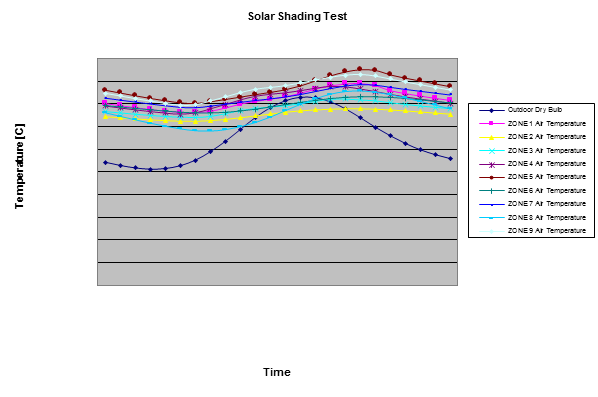
\includegraphics[width=0.9\textwidth, height=0.9\textheight, keepaspectratio=true]{media/image003.png}
\caption{  Example Chart from Standard Output File \protect \label{fig:example-chart-from-standard-output-file}}
\end{figure}
